\documentclass[
%reprint,
%preprint, 
% 11pt,
10pt,
%superscriptaddress,
%groupedaddress,
%unsortedaddress,
%runinaddress,
% frontmatterverbose, 
%preprintnumbers,
%nofootinbib,
%nobibnotes,
%bibnotes,
aps,
pra,
linenumbers,
% twocolumn,
% prl,
% prb,
% prd,
% rmp,
% prstab,
% prstper,
floatfix,
%longbibliography
]{revtex4-2} 
% \usepackage{revquantum}
% new linux font, ignore mono
% \usepackage[mono=false]{libertine} 
% \renewcommand{\baselinestretch}{1.05}
% \usepackage[top=0.7in,left=1in,bottom=1in,right=1in]{geometry}
\usepackage{amsmath,amsthm,amssymb,epsfig,graphicx,mathrsfs,amsfonts,dsfont,bbm}
% \usepackage{bbm} % for \mathbb{1}, but ruins the letter
% \usepackage{unicode-math}
% \DeclareMathOperator*{\argmax}{argmax}
% \DeclareMathOperator*{\argmin}{argmin}
\usepackage{pict2e}
\usepackage[percent]{overpic}
\usepackage{color}
\usepackage{listings}
\usepackage{caption}
% \usepackage{fullpage}
\usepackage[toc,title,titletoc,header]{appendix}
\usepackage{color}
\usepackage{dcolumn}
\usepackage{bm}
\usepackage{hyperref}
\hypersetup{
    citecolor=magenta,
    colorlinks=true,
    linkcolor=blue,
    filecolor=green,      
    urlcolor=cyan,
}
\usepackage[capitalise]{cleveref}
\usepackage{subcaption}
\usepackage{enumitem}
\usepackage{mathtools}
\usepackage{tikz}
\usepackage{tkz-graph} % graph theory
%\usepackage{tikzit}
%\input{path_integral.tikzstyles}
\usepackage{braket}
\usepackage{physics}
% \usepackage{luatex85} % for qcircuit
\usepackage{luatex85,qcircuit}
\usepackage{blkarray}
\usepackage[linesnumbered,ruled,vlined,algosection]{algorithm2e}
\newcommand\mycommfont[1]{\footnotesize\ttfamily\textcolor{blue}{#1}}
\SetCommentSty{mycommfont}

% \setlength\parindent{0pt}
\setcounter{secnumdepth}{3}

\theoremstyle{plain}
\newtheorem{axiom}{Axiom}
\newtheorem{theorem}{Theorem}
\newtheorem{corollary}{Corollary}
\newtheorem{lemma}{Lemma}
\newtheorem{proposition}{Proposition}
\newtheorem{conjecture}{Conjecture} 
\newtheorem{question}{Question} 
\newtheorem{claim}{Claim} 
\theoremstyle{definition}
\newtheorem{definition}{Definition}
\newtheorem{observation}{Observation} 
\newtheorem{fact}{Fact}
\newtheorem{example}{Example}
\newtheorem{remark}{Remark}
\newtheorem{problem}{Problem}


% !TEX root = ./notes.tex

%%%%%%%%%%%%%%%%%%%%%%%%%%%%%%%%%%%%
%%%%%%%%%%%%%% math %%%%%%%%%%%%%%%%
%%%%%%%%%%%%%%%%%%%%%%%%%%%%%%%%%%%%
\newcommand{\calH}{\mathcal{calH}}
\newcommand{\hilbertspace}{\mathcal{H}}
\newcommand{\bigO}{\mathcal{O}}
\newcommand{\lagrangian}{\mathcal{L}}
\newcommand{\VS}{\textrm{VS}}

\newcommand{\realnumber}{\mathbb{R}}
\newcommand{\complexnumber}{\mathbb{C}}
\newcommand{\rationalnumber}{\mathbb{Q}}
\newcommand{\integer}{\mathbb{Z}}
\newcommand{\naturalnumber}{\mathbb{N}}
\newcommand{\numberfield}{\mathbb{F}}

\newcommand{\0}{\mathbf{0}}
\newcommand{\bI}{\mathbf{I}}
\newcommand{\identity}{\mathds{1}}
\newcommand{\midentity}{\mathds{1}}
% \newcommand{\identity}{\mathbb{1}}
\newcommand{\bX}{\mathbf{X}}
\newcommand{\bY}{\mathbf{Y}}
\newcommand{\bepsilon}{\boldsymbol{\epsilon}}

\newcommand{\ii}{\textup{i}}

\newcommand{\floor}[1]{\left\lfloor #1 \right\rfloor}
\newcommand{\ceil}[1]{\left\lceil #1 \right\rceil}

% probability
\newcommand{\probability}{\mathbb{P}}
\newcommand{\variance}{\textup{\textrm{Var}}}
\newcommand{\covariance}{\textup{\textrm{Cov}}}
\newcommand{\expectation}{\mathbb{E}}

% group theory
\newcommand{\group}{\mathbb{G}}
\newcommand{\dihedral}{\mathbb{D}}
\newcommand{\GL}{\mathbb{GL}}
\newcommand{\SL}{\mathbb{SL}}
\newcommand{\Sp}{\textup{Sp}}
% \newcommand{\sp}{\mathfrak{sp}}
\newcommand{\SU}[1]{\textup{SU(#1)}}
\newcommand{\su}[1]{\mathfrak{su}(#1)}
% \renewcommand{\SO}[1]{\textup{SO(#1)}}
% \newcommand{\SO}{\textup{SO}}

% graph theory
\newcommand{\graph}{G}

% matrix and linear algebra
\newcommand{\diag}{\textup{diag}}
% \let\span\relax
% \DeclareMathOperator{\span}{\textup{span}}
% \newcommand{\span}{\textup{span}}
\newcommand{\spn}{\mathop{\mathrm{span}}}
\DeclareMathOperator{\spann}{\textup{span}}
%%%%%%%%%%%%%%%%%%%%%%%%%%%%%%%%%%%%
%%%%%%%%%%%%%%  CS  %%%%%%%%%%%%%%%%
%%%%%%%%%%%%%%%%%%%%%%%%%%%%%%%%%%%%
% cryptography
\newcommand{\gen}{\textsf{Gen}}
\newcommand{\enc}{\textsf{Enc}}
\newcommand{\dec}{\textsf{Dec}}
\newcommand{\mac}{\textsf{Mac}}
\newcommand{\sign}{\textsf{Sign}}
\newcommand{\verfy}{\textsf{Verfy}}
\newcommand{\negl}{\textup{negl}}

% quantum computing
% gates
\newcommand{\cnot}{\textup{\textsc{cnot}}}
\newcommand{\hdm}{\textup{\textsc{h}}}
\newcommand{\tphase}{\textup{\textsc{t}}}
\newcommand{\cphase}{\textup{\textsc{cphase}}}
\newcommand{\swap}{\textup{\textsc{swap}}}
\newcommand{\negate}{\textup{\textsc{not}}}
\newcommand{\QFT}{\textup{QFT}}

% Boolean Functions
\newcommand{\MAJ}{\textup{\textsc{maj}}}
\newcommand{\NOT}{\textup{\textsc{not}}}
\newcommand{\OR}{\textup{\textsc{or}}}
\newcommand{\AND}{\textup{\textsc{and}}}
\newcommand{\NAND}{\textup{\textsc{nand}}}
\newcommand{\EQ}{\textup{\textsc{eq}}}
\newcommand{\IP}{\textup{\textsc{ip}}}
\newcommand{\DISJ}{\textup{\textsc{disj}}}
\newcommand{\Parity}{\textup{\textsc{parity}}}
\newcommand{\Threshold}{\textup{\textsc{thr}}}

\newcommand{\GS}{\textup{\textsc{gs}}}
\newcommand{\dejo}{\textup{\textsc{DeJo}}}
\newcommand{\STAB}{\textup{\textsc{stab}}}

% algorithms
\newcommand{\algo}{\mathcal{A}}
\newcommand{\maxcut}{\textup{\textsc{MaxCut}}}
\newcommand{\sat}{\textup{\textsc{sat}}}
\newcommand{\partition}{\textup{\textsc{Partition}}}
\newcommand{\bosonsample}{\textup{\textsc{BosonSampling}}}

% complexity measures
\newcommand{\vcdim}{\mathsf{VCdim}}
\DeclareMathOperator{\certificate}{\mathsf{Cert}}
\DeclareMathOperator{\s}{\mathsf{s}}
\DeclareMathOperator{\bs}{\mathsf{bs}}
\DeclareMathOperator{\adeg}{\mathsf{\widetilde{deg}}}
% \DeclareMathOperator{\adv}{\mathsf{Adv}}
\DeclareMathOperator{\dqc}{\mathsf{D}}
\DeclareMathOperator{\rqc}{\mathsf{R}}
\DeclareMathOperator{\qqc}{\mathsf{Q}}
\DeclareMathOperator{\cmc}{\mathsf{C}}
\DeclareMathOperator{\rcmc}{\mathsf{RC}}
\DeclareMathOperator{\qcmc}{\mathsf{QC}}
\let\deg\relax
\DeclareMathOperator{\deg}{\mathsf{deg}}
\DeclareMathOperator{\poly}{\textup{poly}}

% complexity classes
\newcommand{\reduceto}{\le_P}
\let\cclass\textup
\let\P\relax
\newcommand{\P}{\cclass{P}}
\newcommand{\PP}{\cclass{PP}}
\newcommand{\NP}{\cclass{NP}}
\newcommand{\sharpP}{\cclass{\#P}}
\newcommand{\coNP}{\cclass{co-NP}}
\newcommand{\PH}{\cclass{PH}}
\newcommand{\NPC}{\cclass{NPC}}
\newcommand{\BQP}{\cclass{BQP}}
\newcommand{\QMA}{\cclass{QMA}}
\newcommand{\PSPACE}{\cclass{PSPACE}}
\newcommand{\BPP}{\cclass{BPP}}

% Optimization
\newcommand{\subjectto}{\textup{subject to  }}

\let\iff\relax
\newcommand{\iff}{\text{ iff }}
\newcommand{\eff}{\textup{eff}}
\newcommand{\st}{\text{ s.t. }}
\newcommand{\otherwise}{\text{otherwise}}
\newcommand{\T}{\intercal}
\newcommand{\OPT}{\textup{OPT}}


\newcommand\vartextvisiblespace[1][.5em]{%
  \makebox[#1]{%
    \kern.07em
    \vrule height.3ex
    \hrulefill
    \vrule height.3ex
    \kern.07em
  }% <-- don't forget this one!
}
\newcommand{\visiblespace}{\vartextvisiblespace}

%%%%%%%%%%%%%%%%%%%%%%%%%%%%%%%%%%%%
%%%%%%%%%%%%% Physics %%%%%%%%%%%%%%
%%%%%%%%%%%%%%%%%%%%%%%%%%%%%%%%%%%%
\newcommand{\zpartition}{\mathcal{Z}}
\newcommand{\llaplacian}{\mathfrak{L}}
\newcommand{\dlagrangian}{\mathcal{L}}
\newcommand{\eaction}{\mathcal{A}}
\newcommand{\action}{\mathcal{S}}
\newcommand{\hhat}{\hat{H}}
\newcommand{\xhat}{\hat{x}}
\newcommand{\phat}{\hat{p}}
\newcommand{\qhat}{\hat{q}}
\newcommand{\nhat}{\hat{n}}
\newcommand{\pihat}{\hat{\pi}}
\newcommand{\phihat}{\hat{\phi}}
\newcommand{\oph}{\mathbf{H}}
\newcommand{\opx}{\mathbf{x}}
\newcommand{\opp}{\mathbf{p}}
\newcommand{\opq}{\mathbf{q}}
\newcommand{\vecx}{\vec{x}}
\newcommand{\vecp}{\vec{p}}
\newcommand{\veck}{\vec{k}}
\newcommand{\vecq}{\vec{q}}
\newcommand{\vbk}{\vb{k}}
\newcommand{\vbs}{\vb{s}}
\newcommand{\vbx}{\vb{x}}
\newcommand{\vbn}{\vb{n}}
\newcommand{\vbp}{\vb{p}}
\newcommand{\vbq}{\vb{q}}
\newcommand{\vbr}{\vb{r}}
\newcommand{\vbe}{\vb{e}}
\newcommand{\vbv}{\vb{v}}
\newcommand{\vbw}{\vb{w}}
\newcommand{\vbB}{\vb{B}}
\newcommand{\vbE}{\vb{E}}
% \newcommand{\acreation}{\hat{a}^\dagger}
% \newcommand{\aannihilation}{\hat{a}}
\newcommand{\acreation}{\hat{a}^\dagger}
\newcommand{\aannihilation}{\hat{a}}
\newcommand{\bcreation}{\hat{b}^\dagger}
\newcommand{\bannihilation}{\hat{b}}
\newcommand{\ccreation}{\hat{c}^\dagger}
\newcommand{\cannihilation}{\hat{c}}
\newcommand{\homega}{\hbar \omega}
\newcommand{\opsigma}{\hat{\bm{\sigma}}}
\newcommand{\hatsigma}{\hat{\sigma}}
\newcommand{\bmhsig}{\bm{\hat{\sigma}}}
\newcommand{\hsig}{\hat{\sigma}}
\newcommand{\si}{\hat{\sigma}_0}
\newcommand{\sx}{\hat{\sigma}_x}
\newcommand{\sy}{\hat{\sigma}_y}
\newcommand{\sz}{\hat{\sigma}_z}
\newcommand{\splus}{\hat{\sigma}_+}
\newcommand{\sminus}{\hat{\sigma}_-}
\newcommand{\px}{\hat{X}}
\newcommand{\py}{\hat{Y}}
\newcommand{\pz}{\hat{Z}}
\newcommand{\pI}{\hat{I}}
\newcommand{\schrodinger}{\textup{Schr\"{o}dinger }}
\newcommand{\tc}{T_c}
\newcommand{\alembertian}{\square}
\newcommand{\vecA}{\vb{A}}
\newcommand{\magfield}{\vb{B}}
\newcommand{\elefield}{\vb{E}}

\newcommand{\deltat}{\Delta t}
\newcommand{\deltatau}{\Delta \tau}

%%%%%%%%%%%%%%%%%%%%%%%%%%%%%%%%%%%%
%%%%%%%%%%%%% Quantum Computing %%%%%%%%%%%%%%
%%%%%%%%%%%%%%%%%%%%%%%%%%%%%%%%%%%%
% \newcommand{\gcommutator}[1]{[[ #1 ]]}
\usepackage{stmaryrd}
\newcommand{\gcommutator}[1]{\llbracket #1 \rrbracket}
\renewcommand{\llaplacian}{\hat{\mathfrak{L}}}
%\newcommand{\zpartition}{\mathcal{Z}}
\newcommand{\hamiltonian}{\hat{H}}
\newcommand{\kernel}{k}
\newcommand{\ew}{\hat{W}}
\newcommand{\ghz}{\text{GHZ}}
\newcommand{\jsd}{D_\text{JS}}
\newcommand{\kl}{D_\text{KL}}
\newcommand{\shadow}{\text{shadow}}
\newcommand{\noise}{\text{noise}}
\newcommand{\ob}{\hat{O}}
\newcommand{\U}{\hat{U}}
\newcommand{\subgroup}{\mathbb{H}}
\newcommand{\ppartition}{\mathcal{P}}
\newcommand{\dm}{\rho}
\newcommand{\oracle}{\hat{O}}
\newcommand{\D}{\mathcal{D}}
\newcommand{\proj}{\hat{P}}
%\newcommand{\deltat}{\Delta t}
%\newcommand{\deltatau}{\Delta \tau}
\newcommand{\cz}{\textup{\textsc{cz}}}
\newcommand{\cx}{\textup{\textsc{cx}}}
\newcommand{\toffoli}{\textup{\textsc{toffoli}}}
\newcommand{\lleft}{\leftarrow}
\newcommand{\rright}{\rightarrow}
\newcommand{\intinf}{\int_{-\infty}^{\infty}}

% disable subsections and subsubsections in the TOC
\makeatletter
%\def\l@subsection#1#2{}
\def\l@subsubsection#1#2{}
\makeatother

\begin{document}
%%%%%%%%%%%%%%%%%%%
\title{Towards efficient entanglement structure detection}
\author{Jue Xu}
\email{juexu@cs.umd.edu}
\author{Qi Zhao}
\email{email}
% \affiliation{Department of Computer Science, University of Maryland, College Park.}
\date{\today}
%%%%%%%%%%%%%%%%%%%
% \vspace{10mm}
\begin{abstract}
	Verification (detection) of entanglement structure is an indispensable step for practical quantum computation (communication).
	In this work, we compare complexity and performance of several recently-developed methods, including entanglement witness methods, shadow tomography, classical machine learning, and quantum algorithms (circuits).
	illustrate the advantages and limitations of machine learning and quantum algorithms.
\end{abstract}

\maketitle
% \setcounter{tocdepth}{0}
 \tableofcontents
% \newpage

%%%%%%%%%%%%%%%Content%%%%%%%%%%%%%%%
\section{Introduction}
Entanglement \cite{horodeckiQuantumEntanglement2009} is the key ingredient of quantum computation \cite{}, quantum communication \cite{}, and quantum cryptography \cite{}.
It is essential to benckmark (characterize) multipartite entanglement structures of target states.
We review the recently developed methods: entanglement witness \cite{zhouDetectingMultipartiteEntanglement2019}, shadow tomography \cite{huangPredictingManyProperties2020}, classical machine learning \cite{huangPowerDataQuantum2021}, and quantum (variational/circuit) algorithms \cite{quekMultivariateTraceEstimation2022}.

\section{Preliminaries}
% \subsection{Related works}
% \subsection{Notations}
Notations:
The (classical) training data (for supervised learning) is a set of $m$ data points $\qty{(\vbx^{(i)}, y^{(i)})}^{m}_{i=1}$ 
where each data point is a pair $(\vbx,y)$.
Normally, the input (e.g., an image) $\vbx:= (x_1,x_2,\dots,x_d) \in \realnumber^d$  is a vector where $d$ is the number of \emph{features}
and its \emph{label} $y\in\Sigma$ is a scalar with some discrete set $\Sigma$ of alphabet/categories. 
For simplicity and the purpose of this paper, we assume $\Sigma=\qty{-1,1}$ (binary classification).

% Notations: 
a graph $\graph=(V,E)$ is described by vertices $V$ and edges $E$.
denote a group by $\group$ and a subgroup $\subgroup$. 
The hats on the matrices such as $\hat{A}$, $\hamiltonian$, $\dm$ (omitted), $\ob$, $\ew$, emphasize that they play the roles of operators.
Denote vector (matrix) $\vbx$, $\vb{K}$ by boldface font.

For specific purpose, we use different basis (representations) for quantum states.
One is the computational basis $\qty{\ket{z}}$ with $z\in \qty[2^n]$ where $n$ is the number of qubits,
while another useful one is the binary representation of computational basis $\qty{\ket{\vbx}\equiv\ket{x_1,x_2,\dots,x_n}}$ with $x_j\in \qty{0,1}$. 
For simplicity, we let $N \equiv 2^n$ and $\ket{\vb{0}}\equiv\ket{0^n} \equiv\ket{0}^{\otimes n}$ if no ambiguity.
$\ket{+}: = (\ket{0}+\ket{1})/\sqrt{2} $

\subsection{Entanglement detection}
Large scale entanglement is the (main) resource of quantum advantages in quantum computation and communication.
\begin{definition}[Entangled state]\label{def:entangled_state}
	Consider a $n$-partite (subsystem) system $\hilbertspace=\bigotimes_i^n \hilbertspace_i$,
	separable states or product states are i.e.,
	\begin{equation}
		\ket{\Psi} = \bigotimes_i \ket{\psi_i}
	\end{equation}
	entangled pure state is a quantum state that cannot be written as a (tensor) product state (inseparable). 
	For (generalize) mixed states, a mixed entangled state is a convex combination of entangled pure state, that is
	\begin{equation}
		\rho = \sum_i p_i\op{\Psi_i},\forall i,p_i\ge 0, \sum_i p_i =1
	\end{equation}
		...
\end{definition}
% \begin{example}
% 	Bell states
% \end{example}
Many methods [...] have been developed to determine whether a state is separable.
\begin{definition}[Bipartite state]
\end{definition}

% \subsubsection{entanglement measures}
Instead of qualitatively determining entanglement, quantify entanglement
\begin{definition}[Schmidt coefficient/rank/measure]
	% Schmidt decomposition	
	consider the following pure state on system AB, written in Schmidt form:
	\begin{equation}
		\ket{\psi} = \sum_i \sqrt{p_i} \ket{\phi_i^A}\otimes\ket{\phi_i^B}
	\end{equation}
	where $\qty{\ket{\psi_1^A}}$ is a basis for $\hilbertspace_A$ and ...
	The strictly positive values $\sqrt{p_i}$ in the Schmidt decomposition are its \emph{Schmidt coefficients}. 
	The number of Schmidt coefficients, counted with multiplicity, is called its \emph{Schmidt rank}, or Schmidt number.
	Schmidt measure
\end{definition}
\begin{example}
	The Schmidt measure for any multi-partite \nameref{exm:ghz} states is 1.
	... 1D, 2D, 3D-cluster state is $\floor{\frac{N}{2}}$.
	.. of tree is the size of its minimal vertex cover.
\end{example}
% \begin{remark}
% 	When a bipartite vector is written in the Schmidt basis, it is very easy to compute the partial trace of either subsystem	
% 	\begin{equation}
% 		\Tr_B(\op{\psi}) = \sum_i p_i \op{\phi_i^A}
% 	\end{equation}
% \end{remark}
\begin{definition}[entropy]\label{def:entropy}
	% entanglement entropy
	In quantum mechanics (information), the von Neumann \emph{entropy} of a density matrix is $H_N(\dm): = -\Tr(\dm \log \dm)=-\sum_i\lambda_i\log(\lambda_i)$;
	In classical information (statistical) theory, the Shannon entropy of a probability distribution $P$ is  $H_S(P):= -\sum_i P(x_i) \log P(x_i)$.
	relative entropy (\nameref{def:divergence})
\end{definition}

\subsubsection{entanglement structures}
For multipartite quantum systems, it is crucial to identify not only the presence of entanglement but also its detailed structure.
An identification of the entanglement structure may thus provide us with a hint about where imperfections in the setup may occur, as well as where we can identify groups of subsystems that can still exhibit strong quantum-informationprocessing capabilities.
To benchmark our technological progress towards the generation of largescale genuine multipartite entanglement, it is thus essential to determine the corresponding entanglement depth.

Given a $n$-qubit quantum system and its partition into $m$ subsystems, the \emph{entanglement structure} indicates how the subsystems are entangled with each other.
In some specific systems, such as distributed quantum computing[] quantum networks[] or atoms in a lattice, the geometric configuration can naturally determine the system partition.

\begin{definition}[genuine entangled]\label{def:genuinely_entangled}
	A state possesses \emph{genuine multipartite entanglement} (GME) if it is outside of $S_2$, and is (fully) $n$-separable if it is in $S_n$.
	A state possesses $\ppartition$-genuine entanglement if it is outside of $S_b^\ppartition$.
	A state $\dm$ possesses $\ppartition$-genuine entanglement iff $\dm\notin S_b^\ppartition$.
\end{definition}
% \begin{remark}
	Compared with genuine entanglement, multipartite entanglement structure still lacks a systematic exploration, due to the rich and complex structures of $n$-partite system.
	Unfortunately, it remains an open problem of efficient entanglement-structure detection of general multipartite quantum states.
% \end{remark}
\begin{definition}[Multipartite state]
	denote the partition $\ppartition_m = \qty{A_i}$
	and omit the index $m$ when it is clear from the context.
\end{definition}
define fully- and biseparable states with respect to a \emph{specific partition} $\ppartition_m$
\begin{definition}[fully separable]\label{def:fully_separable}
	An $n$-qubit pure state $\ket{\psi_f}$ is \emph{fully separable} \iff .
	An $n$-qubit pure state $\ket{\psi_f}$ is \emph{P-fully separable} \iff it can be written as 
	$\ket{\psi_f}=\otimes_i^m \ket{\phi_{A_i}}$.
	An $n$-qubit mixed state $\dm_f$ is P-fully separable $\iff$ it can be decomposed into a convex mixture of P-fully separable pure states 
	% \begin{equation}
	% 	\dm_f = \sum_i p_i \op{\psi_f^i}, (\forall i) ( p_i\ge 0, \sum_i p_i = 1) .
	% \end{equation}
	P-bi-separable... $S_f^P \subset S_b^P$
\end{definition}
By going through all possible partitions, one can investigate higher level entanglement structures, such as entanglement intactness (non-separability), which quantifies how many pieces in the $n$-partite state are separated.

\begin{remark}
	P-... can be viewed as generalized versions of regular fully separable, biseparable, and genuinely entangled states, respectively.
	In fact, when $m=n$, these pairs of definitions are the same.
	By definitions, one can see that if a state is $P_m$-fully separable, it must be m-separable. Of course, an m-separable state might not be $P_m$-fully separable, for example, if the partition is not properly chosen.
	Moreover, for some systems, such as distributed quantum computing, multiple quantum processor, and quantum network, natural partition exists due to the system geometric configuration. Therefore, it is practically interesting to study entanglement structure under partitions.
\end{remark}
entanglement structure measures
\begin{definition}[Entanglement intactness, depth]
	the entanglement intactness of a state $\dm$ to be $m$, \iff $\dm\notin S_{m+1}$ and $\dm\in S_m$.
	$k$-producible
\end{definition}

% \begin{remark}
	When the entanglement intactness is 1, the state is \nameref{def:genuinely_entangled}; and when the intactness is $n$, the state is \nameref{def:fully_separable}.
% \end{remark}
\begin{example}[GHZ]\label{exm:ghz}
	bipartite: Bell states;
	nontrivial multipartite: tripartite.
	GHZ state: $\ket{\ghz}:=\frac{1}{\sqrt{2}}(\ket{0}^{\otimes n} + \ket{1}^{\otimes n} )$ (eight-photon) produce the five different entangled states (one from each entanglement structure): 
	\begin{equation*}
		\ket{\ghz_8},\ket{\ghz_{62}},\ket{\ghz_{44}},\ket{\ghz_{422}},\ket{\ghz_{2222}}.
	\end{equation*}
	% W state
	Schmidt rank, PPT criteria
\end{example}

\begin{figure}[!ht]
	\centering
	\begin{subfigure}{0.3\textwidth}
		\centering
		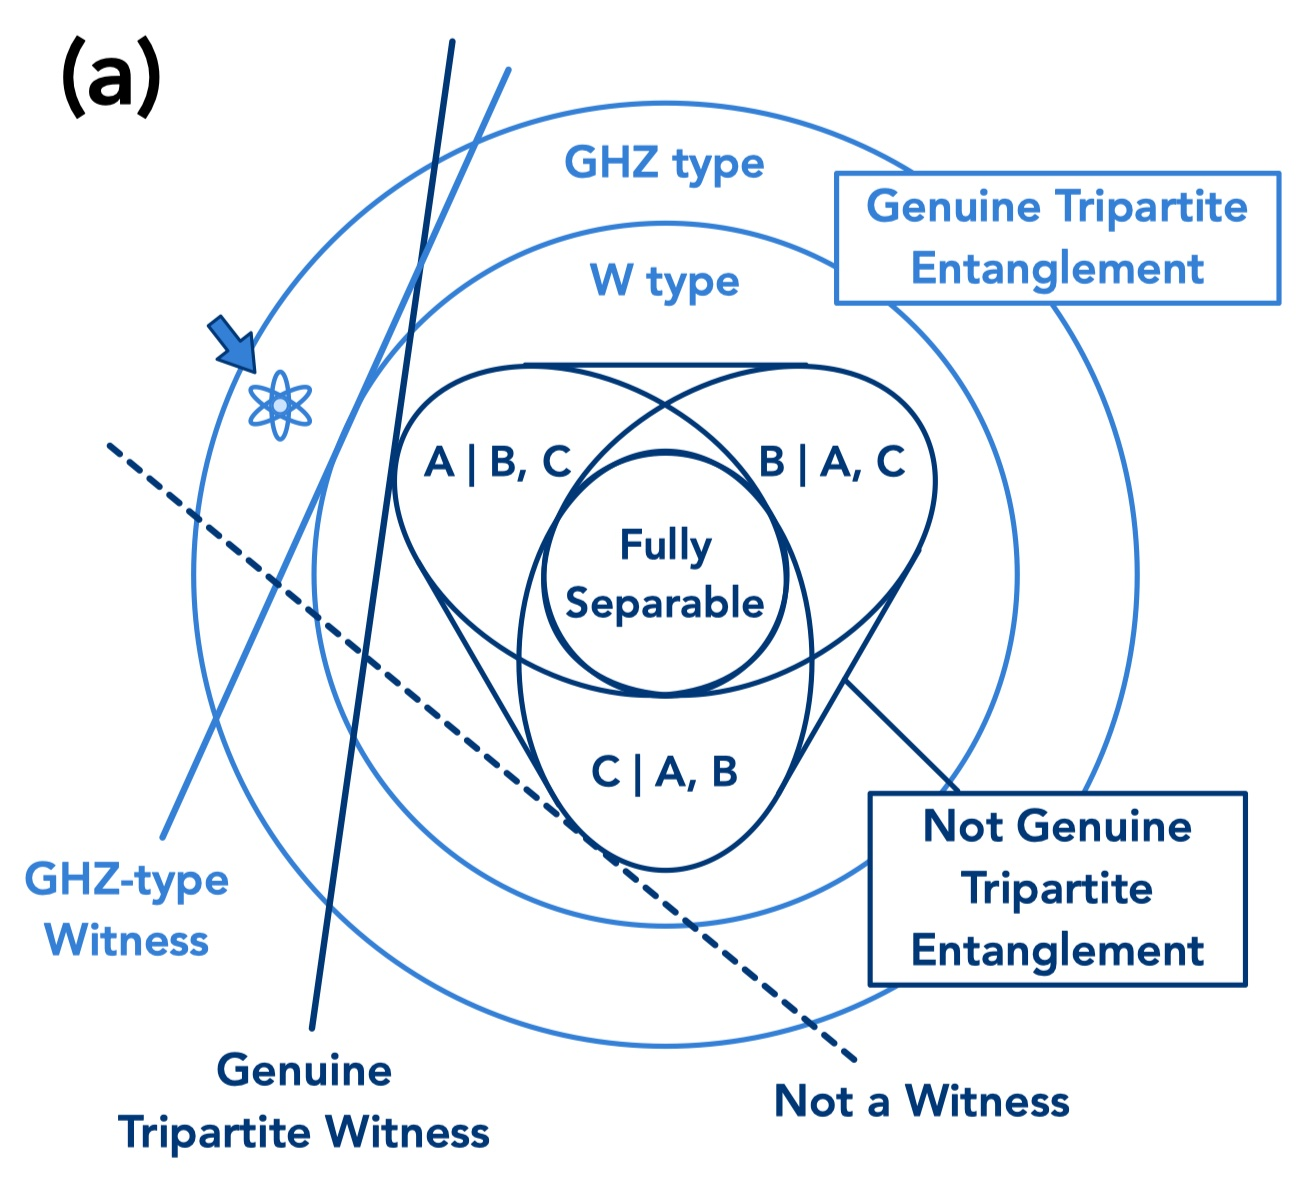
\includegraphics[width=.9\linewidth]{gme.jpg}
	\end{subfigure}
	\begin{subfigure}{0.3\textwidth}
		\centering
		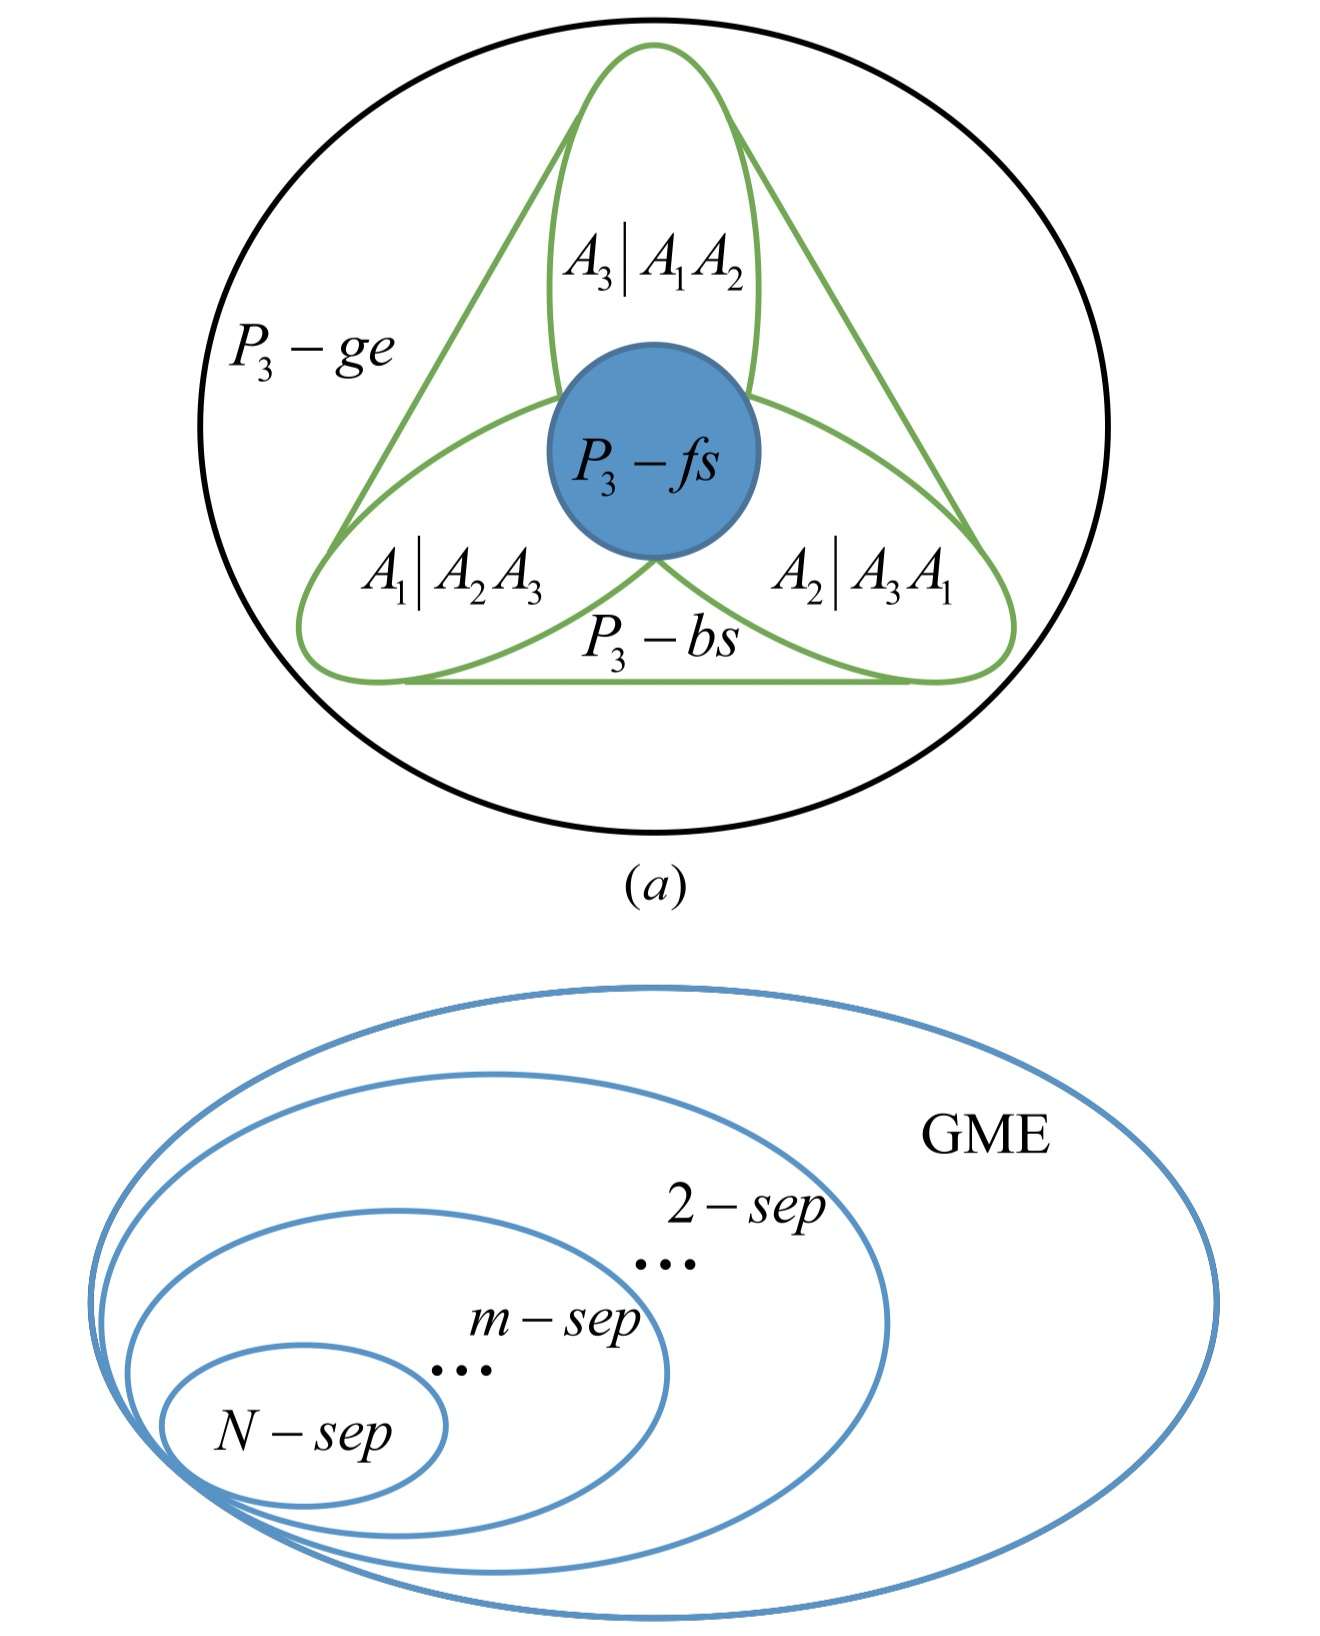
\includegraphics[width=.8\linewidth]{sep.jpg}
	\end{subfigure}
	\begin{subfigure}{0.35\textwidth}
		\centering
		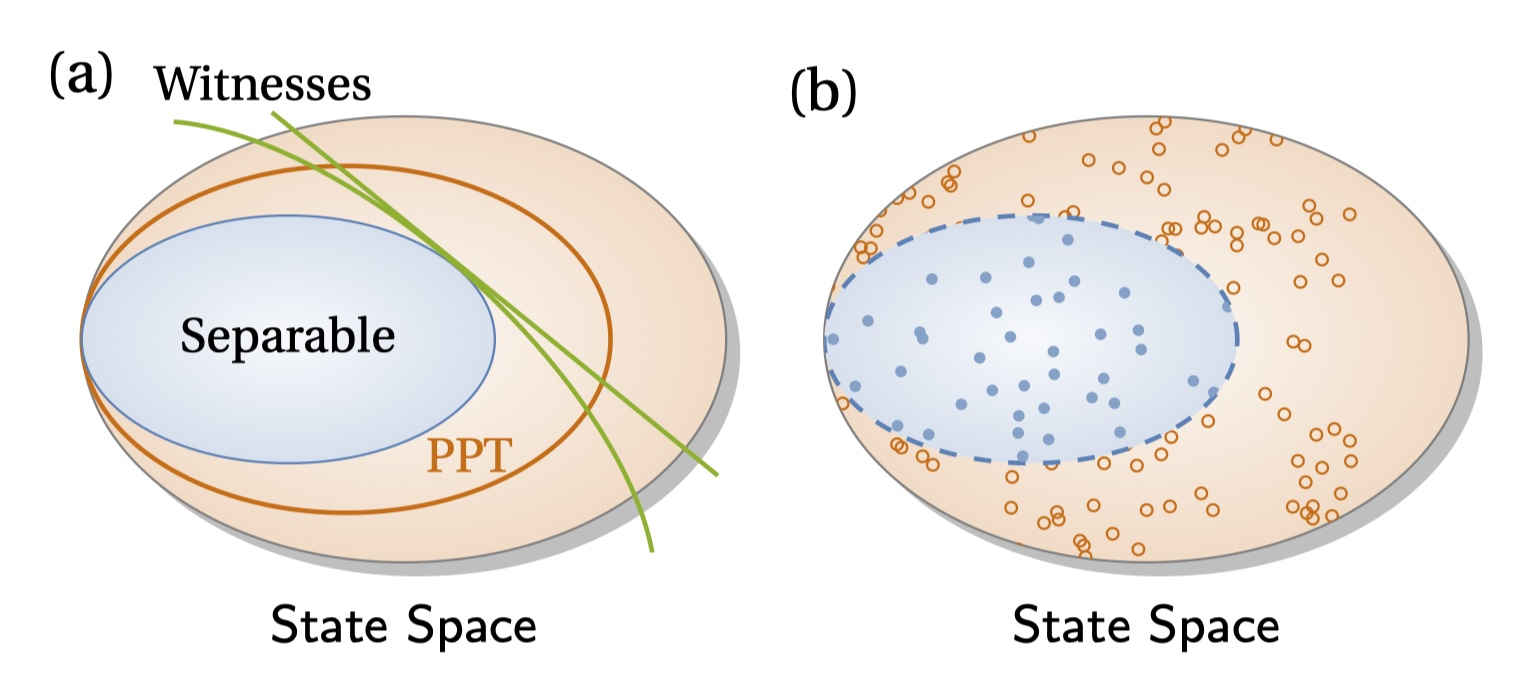
\includegraphics[width=.9\linewidth]{ppt.jpg}
	\end{subfigure}
	\caption{(a) entanglement witness, PPT criteria, SVM (kernel)?. (c) convex hull... }
	\label{fig:entangle}
\end{figure}

\subsubsection{Entanglement witness}\label{sec:entanglement_witness}
\begin{theorem}[\cite{gurvitsClassicalDeterministicComplexity2003}]
	% The problem of determining whether a given quantum state is entangled lies at the heart of quantum information processing, which is an NP-hard problem in general.
	The weak membership problem for the convex set of separable normalized bipartite density matrices is NP-Hard.
	\textbf{Input}: ??
	% \begin{itemize}
	% 	\item \textbf{Input}: ??
	% 	\item \textbf{Output}: ??
	% \end{itemize}
\end{theorem}
\begin{question}
	specific cases? approximately correct? quantum computation? machine learning (data)?
\end{question}

\begin{theorem}[PPT criterion]
	the positive partial transpose (PPT) criterion, saying that a separable state must have PPT?.
	Note, it is only necessary and sufficient when $d_A d_B \le 6$.
\end{theorem}
see \cref{fig:entangle}
\begin{definition}[entanglement witness]\label{def:entanglement_witness}
	Given an (unknown) quantum state (density matrix) $\dm$, the \emph{entanglement witness} $\ew$ is an obseverable such that
	\begin{equation}
		\Tr(\ew\dm) \ge 0 , \forall \text{ separable };\quad
		\Tr(\ew\dm) < 0 , \text{ for some entangled }
	\end{equation}
\end{definition}
It is natural to ask nonlinear entanglement witness \cite{guhneNonlinearEntanglementWitnesses2006}  
\nameref{def:kernel} ML
\begin{proposition}
	Given a state $\ket{\psi}$,
	the \nameref{def:entanglement_witness} operator $\ew_{\psi}$ can witness genuine multipartite entanglement near $\ket{\psi}$
	% \nameref{def:genuinely_entangled}
	\begin{equation}
		\ew_{\psi} = \frac{5}{8}\identity - \op{\psi} 
	\end{equation}
	with $\expval{\ew_{\psi}}\ge 0$ for any separable state in $S_b$.
\end{proposition}
If the \nameref{def:fidelity} of the prepared state $\dm_{\text{pre}}$ with the target state $\ket{\psi}$, i.e., $\Tr(\dm_{pre}\op{\psi})$, exceeds $5/8$, $\dm_{pre}$ possesses GME.
It is generally difficult to evaluate the quantity $\Tr(\dm_{pre}\op{\psi})$ by the direct projection on $\ket{\psi}$, as it is an entangled state.

\begin{problem}[Entanglement witness with prior]
	% \cite{zhouDetectingMultipartiteEntanglement2019}
	with/out prior knowledge
	\begin{itemize}
		\item \textbf{Input}: a \textbf{known} state $\ket{\psi}$, with noise
		\item \textbf{Output}: separable or not ???
		(decision problem?? find problem)
	\end{itemize}
\end{problem}

\subsubsection{Graph state}
graph state is an important (large?) class of multipartite states in quantum information.
Typical graph states include cluster states, \nameref{exm:ghz} states, and the states involved in error correction (toric code?).
% cluster state is the special case of graph state.
It worth noting that 2D cluster state is the universal resource for the measurement based quantum computation (MBQC) \cite{briegelMeasurementbasedQuantumComputation2009}.
\begin{definition}[graph state]\label{def:graph_state}
	Given a (undirected, unweighted) graph $G=(V,E)$, a graph state is constructed as 
	from the initial state $\ket{+}^{\otimes n}$ corresponding to $n$ vertices.
	Then, apply controlled-Z gate to every edge, that is 
	\begin{equation}
		\ket{G}=\prod_{(i,j)\in E}\textsf{cZ}_{(i,j)} \ket{+}^{\otimes n}
	\end{equation}
	% \begin{itemize}
	% 	\item vertices: $\ket{+}^{\otimes n}$
	% 	\item edges: apply controlled-Z to every edge,
	% 	that is $\ket{G}=\prod_{(i,j)\in E}\textsf{cZ}_{(i,j)} \ket{+}^{\otimes n}$
	% \end{itemize}
\end{definition}
\begin{remark}
	An $n$-partite graph state can also be uniquely determined by $n$ independent stabilizers, 
	$S_i:= X_i \bigotimes_{j\in n}Z_j$, 
	which commute with each other and $\forall i,S_i\ket{G}=\ket{G}$.??
	The graph state is the unique eigenstate wtih eignevalue of +1 for all the $n$ stabilizers.
	As a result, a graph state can be writteb as a product of stailizer projectors, $\op{G}=\prod_{i=1}^n \frac{S_i +\identity}{2}$.
	stabilizer formalism?; 
\end{remark}
% \begin{question}
% \end{question}
\begin{example}[graph states]
	\nameref{exm:ghz} (star); complete graph, hypercube, Petersen graph; cluster state
	\begin{figure}[!ht]
		\centering
		\begin{subfigure}{0.3\textwidth}
		\centering
		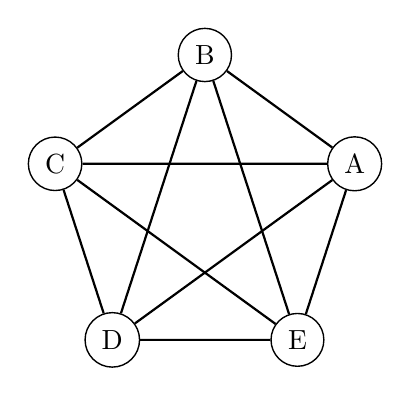
\begin{tikzpicture}[rotate=18]
			\SetGraphUnit{2} 
			\GraphInit[vstyle=Normal] 
			% \renewcommand*{\VertexInnerSep}{8pt} \renewcommand*{\EdgeLineWidth}{3pt} \renewcommand*{\VertexBallColor}{blue!50} 
			\Vertices{circle}{A,B,C,D,E} 
			\Edges(A,B,C,D,E,A,C,E,B,D,A) 
		\end{tikzpicture}
		\caption{complete graph $K_5$}
		\end{subfigure}
		\begin{subfigure}{0.3\textwidth}
		\centering
		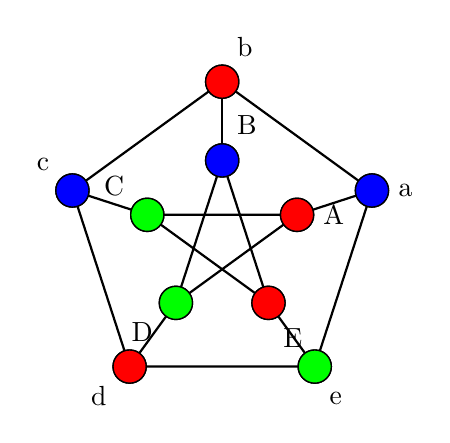
\begin{tikzpicture}[rotate=18,scale=1.0]
			\SetGraphUnit{1} 
			\GraphInit[vstyle=Welsh] 
			% \renewcommand*{\VertexLineWidth}{2pt}
			% \renewcommand*{\VertexInnerSep}{8pt} 
			% \renewcommand*{\EdgeLineWidth}{3pt} 
			% \renewcommand*{\VertexBallColor}{blue!50} 
			\Vertices{circle}{A,B,C,D,E} 
			\Edges(A,D,B,E,C,A) 
			\SetGraphUnit{2} 
			\Vertices{circle}{a,b,c,d,e} 
			\Edges(a,b,c,d,e,a) 
			\Edges(A,a)
			\Edges(B,b)
			\Edges(C,c)
			\Edges(D,d)
			\Edges(E,e)
			\AddVertexColor{red}{b,d,A,E} 
			\AddVertexColor{blue}{c,B,a}
			\AddVertexColor{green}{C,D,e}
		\end{tikzpicture}
		% \caption{A 3-coloring of the Petersen graph}
		\caption{Petersen graph}
		\end{subfigure}
		\begin{subfigure}{0.3\textwidth}
		\centering
		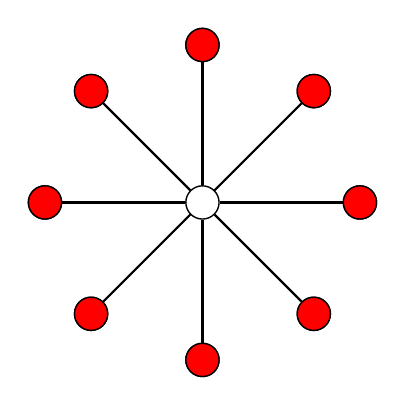
\begin{tikzpicture}[rotate=90] 
			\GraphInit[vstyle=Hasse] 
			\Vertices[unit=2]{circle}{A,B,C,D,E,F,G,H} 
			\coordinate (Z) at (intersection of A--E and B--F); 
			\Vertex[Node]{Z}% voir option node
			\Edges(A,Z)
			\Edges(B,Z)
			\Edges(C,Z)
			\Edges(D,Z)
			\Edges(E,Z)
			\Edges(F,Z)
			\Edges(G,Z)
			\Edges(H,Z)
			\AddVertexColor{red}{A,B,C,D,E,F,G,H} 
		\end{tikzpicture}
		\caption{star - GHZ}
		\end{subfigure}
	\end{figure}
\end{example}
% \begin{question}
% 	efficient? meaningful encoding of graph data/input??
% 	Hamiltona cycle of a graph state? vertex cover
% \end{question}
% \begin{problem}[Entanglement structure detection]
% \end{problem}
\begin{problem}[Certify entanglement]
	Multipartite entanglement-structure detection
	\begin{itemize}
		\item \textbf{Input}: Given a state close to a \textbf{known} (general multipartite) state $\ket{\psi}$,
		certain partition?
		\item \textbf{Output}: the certified lower-order entanglement among several subsystems could be still useful for some quantum information tasks.
		entanglement structure
	\end{itemize}
\end{problem}
\begin{remark}
	The entanglement \nameref{def:entropy} $S( \dm_A )$ equals the rank of the adjacency matrix of the underlying bipartite graph, which can be efficiently calculated.
\end{remark}
\begin{proposition}[\cite{zhouDetectingMultipartiteEntanglement2019}]
	Given a graph state $\ket{G}$ and a partition $\mathcal{P}=\qty{A_i}$, the \nameref{def:fidelity} between $\ket{G}$ and any \nameref{def:fully_separable} is upper bounded by
	\begin{equation}
		\Tr(\op{G} \dm_f) \le \min_{\qty{A,\bar{A}}} 2^{-S(\dm_A)}
	\end{equation}
	where $S(\dm_A)$ is the von Neumann \nameref{def:entropy} of the reduced density matrix $\dm_A=\Tr_{\bar{A}}(\op{G})$.
\end{proposition}
\begin{theorem}
	k local measurements. Here, k is the chromatic number of the corresponding graph, typically, a small constant independent of the number of qubits.
\end{theorem}
\begin{proposition}[Entanglement of graph state]
	\cite{heinEntanglementGraphStates2006}.
	witness; bounds; graph property? vertex cover?
	Hamiltona cycle of a graph state? 
\end{proposition}
generalize \cite{zhangEfficientEntanglementGeneration2021}
stabilizer state, neural network state \cite{gaoEfficientRepresentationQuantum2017}?
\begin{proposition}[Entanglement witness for graph state]
\end{proposition}
\begin{proposition}[Bounds to the Schmidt measure of graph states]
	For any graph state $\ket{G}$, the Schmidt measure $E_A$ is bounded from below by the maximal Schmidt rank $SR_{\max}$ and from above by the Pauli persistency PP or the minimal vertex cover, i.e.
	\begin{equation}
		SR_{\max} (G) \le E_S(\ket{G}) \le PP(G) \le VC(G).
	\end{equation}
	???
\end{proposition}


\subsection{Shadow tomography}
% \label{sec:shadow_tomography}
Intuitively, a general tomography \cite{altepeterPhotonicStateTomography2005} that extract (recover) all information about a state requires exponential copies (samples/measurements).
\begin{problem}[full tomography]\label{prm:full_tomography}
	In contrast to \nameref{prm:shadow_tomography}, we refer to \emph{full tomography} here
	\begin{itemize}
		\item \textbf{Given (Input):} a \textbf{unknown} $N$-dimensional mixed state $\dm$
		\item \textbf{Goal (Output):} a complete description? of $\dm$ (decomposition coefficients) with error?
	\end{itemize}
\end{problem}
\begin{theorem}[lower bound of \nameref{prm:full_tomography}?\cite{haahSampleoptimalTomographyQuantum2017}]
	Known fundamental lower bounds [66, 73] state that classical shadows of exponential size (at least) $T = \Omega( 2^n / \epsilon^2)$ are required to $\epsilon$-approximate $\dm$ in trace \nameref{def:distance}.
\end{theorem}
\begin{definition}[fidelity]\label{def:fidelity}
	Given a pair of states (target and real), 
	fidelity $F(\rho,\rho') : = \Tr(\sqrt{\sqrt{\rho}\rho'\sqrt{\rho}})$
	% \begin{equation}
	% 	F(\ket{\psi},\ket{\psi'}) :=
	% \end{equation}
	% \begin{equation}
	% 	F(\rho,\rho') : = \Tr \sqrt{\sqrt{\rho}\rho'\sqrt{\rho}}
	% \end{equation}
\end{definition}
\begin{definition}[distance]\label{def:distance}
	trace distance $d_{\tr}(\rho,\rho') : = \frac{1}{2} \norm{\rho-\rho'}_1$
	% \begin{equation}
	% 	d_{tr}(\rho,\rho') : = \frac{1}{2} \norm{\rho-\rho'}_1
	% \end{equation}
	% relation
	% \begin{equation}
	% 	1-F\le D_{tr} \le \sqrt{1-F^2}
	% \end{equation}
\end{definition}
\begin{definition}[norm]\label{def:norm}
	Schatten p-norm $\norm{x}_p:= (\sum_i \abs{x_i}^p)^{1/p}$.
	Euclidean norm $l_2$ norm;
	Spectral (operator) norm ;
	Trace norm $\norm{A}_{\Tr}\equiv\norm{A}_{1}:=\Tr(\sqrt{A^\dagger A})$, $p=1$;
	Frobenius norm $\norm{A}_{F}:=\sqrt{\Tr(A^\dagger A)}$, $p=2$;
	Hilbert-Schmidt norm $\norm{A}_{HS}:=\sqrt{\sum_{i,j} A_{ij}^2 }$
\end{definition}
\begin{problem}[Fidelity estimate]
	defined as follows
	\begin{itemize}
		\item \textbf{Input}: Given two density matrices $\dm$ and $\dm'$, 
		\item \textbf{Output}: \nameref{def:fidelity} with error $\epsilon$
	\end{itemize}
\end{problem}
\begin{problem}[trace estimation]\label{prm:trace_estimation}
	defined as follows
	\begin{itemize}
		\item \textbf{Input}: Given an observable $\ob$ and a mixed state $\dm$ in density matrix,
		\item \textbf{Output}: the expectation value $\Tr(\ob \dm) = $ with error $\epsilon$ (trace \nameref{def:distance})
	\end{itemize}
		The task of estimating quantities like 
		\begin{equation}
			\Tr(\rho_1 \cdots \rho_m)
			\tag{multivariate traces}
		\end{equation}
		given access to copies of the quantum states $\rho_1$  through $\rho_m$.
\end{problem}
Nevertheless, we usually only need specific properties of a target state rather than all information about the state.
This enables the possibility to .
Inspired by Aaronson's shadow tomography \cite{aaronsonShadowTomographyQuantum2018}, Huang et. al \cite{huangPredictingManyProperties2020}
\begin{problem}[shadow tomography]\label{prm:shadow_tomography}
	\emph{shadow tomography}
	\begin{itemize}
		\item \textbf{Given (Input):} an \textbf{unknown} $N$-dimensional mixed state $\rho$, $M$ known 2-outcome measurements $E_1,\dots,E_M$
		\item \textbf{Goal (Output):} estimate $\probability[E_i \text{ accept } \dm]$ to within additive error $\epsilon$, $\forall i\in [M]$, with $\ge 2/3$ success probability
	\end{itemize}
\end{problem}
\begin{theorem}[\cite{aaronsonShadowTomographyQuantum2018}]\label{thm:shadow_tomography}
	It is possible to do \nameref{prm:shadow_tomography} using $\tilde{\bigO}(\frac{\log^4 M\cdot \log N}{\epsilon^4})$ copies. [no construction algorithm?]
	sample complexity lower bound $\Omega(\log (M) \cdot \epsilon^{-2})$, 
\end{theorem}
random Pauli measurements
\begin{definition}[classical shadow]\label{def:classical_shadow}
	classical shadow
	\begin{equation}
		\dm_{cs} = \mathcal{M}^{-1} \qty(U^\dagger \op{\hat{b}} U)
	\end{equation}
\end{definition}
predict linear function with classical shadows
\begin{equation}
	o_i = \Tr(O_i \dm_{cs})
	\text{ obeys }
	\expectation[o] =\Tr(O_i \dm)
\end{equation}
The classical shadow attempts to approximate this expectation value by an empirical average over $T$ independent samples, much like Monte Carlo sampling approximates an integral.
% \begin{remark}
The classical shadow size required to accurately approximate all reduced $r$-body density matrices scales exponentially in subsystem size $r$, but is independent of the total number of qubits $n$.
% \end{remark}

\begin{algorithm}[H]
    \DontPrintSemicolon
    \SetKwInOut{Input}{input}
    \SetKwInOut{Output}{output}
    \Input{a density matrix $\dm$, ..}
    \Output{classical shadow}
    \BlankLine
    \For{ $i = 1,2, \ldots, m$} {
        random Pauli measurements \tcp*{a comment}
        % \tcc{comment in a new line}
    {\Return "?"}
    }
    \Return ?
    \caption{Shadow tomography}
    \label{alg:classical_shadow}
\end{algorithm}
\begin{lemma}
	the variance
	\begin{equation}
		\variance[o] = \expectation[(o-\expectation[o])^2]
		\le \norm{O - \frac{\Tr(O)}{2^n} \identity}^2_{\shadow}
	\end{equation}
\end{lemma}
sample complexity
\begin{equation}
	N_{tot} = \bigO \qty(
		\frac{\log (M)}{\epsilon^2} \max_{1\le i\le M} 
		\norm{O_i - \frac{\Tr(O_i)}{2^n} \identity}^2_{\shadow}
	)
\end{equation}
\begin{theorem}[Pauli/Clifford measurements]
	additive error $\epsilon$, $M$ arbitrary $k$-local linear function $\Tr(\ob_i\dm)$,
	% lower bound
	$\Omega(\log(M) 3^k/\epsilon^2)$ copies of the state $\dm$.
\end{theorem}

\section{Classical, data-powered, and quantum algorithms}
We consider the problem 
\begin{problem}[?data]
	problem without training data
	\begin{itemize}
		\item \textbf{Input}: a graph $\graph$ encoding in a graph state $\ket{\graph}$
		\item \textbf{Output}: entanglement structure
	\end{itemize}
\end{problem}
with training data: \textbf{features}: classical shadow? raw data? quantum data, label: entangled?
% \begin{itemize}
% 	\item \textbf{features}: classical shadow?
% 	\item label: 
% \end{itemize}

\subsection{Quantum-classical (ML) hybrid method}
\subsubsection{Classical machine learning}\label{sec:classical_machine_learning}
separability classifier by neural network \cite{luSeparabilityEntanglementClassifierMachine2018}.
rigorous quantum advantage of quantum kernel method in SVM \cite{liuRigorousRobustQuantum2021}.
classical machine learning with \nameref{def:classical_shadow} \cite{huangProvablyEfficientMachine2021}.


\begin{remark}
	input encoding: 
	\begin{itemize}
		% \item qubit (basic) encoding?: given a vector $\vb{z}\in\integer^d$, 
		% $\ket{\vb{z}}=\bigotimes_i^d \ket{\vbx_i}$ where $\vbx_i$ is the binary representation of $z_i$,
		% need $\bigO(d\cdot \log(\max(z_i)))$ (not space efficient)

		% \item phase encoding?

		\item amplitude encoding: given a normalized vector $\vbx\in\realnumber^d$, the quantum state $\ket{\vbx}=\sum_z^d x_z\ket{z}$. 
		need $\log(d) $ qubits for a data point; dequantization \cite{tangQuantumPrincipalComponent2021}

		\item graph state encoding: \nameref{def:graph_state}, discrete, efficient? space (time), isomorphism?

		\item quantum data $\ket{\psi}$ or $\dm$: quantum state from real-world experiments or quantum circuits $\U$

		% \item (quantum) oracle: $\oracle \ket{i,a}=\ket{i,a+x_i}$; quantum oracle: unitary and controlled unitary
	\end{itemize}
\end{remark}
nonlinear boundary. map to a higher dimensional (feature) space, in which data is linearly separable.
\begin{definition}[kernel]\label{def:kernel}
	In general, the kernel function $\kernel:\mathcal{X}\times \mathcal{X} \to \realnumber$ measures the similarity between two input data points by an inner product
	\begin{equation}
		\kernel (\vbx,\vbx') : = \expval{\phi(\vbx),\phi(\vbx')}
	\end{equation}
	If the input $\vbx\in \realnumber^d$, the feature map $\phi(\vbx): \realnumber^d\to \realnumber^n$ ($n > d$) from a low dimensional space to a higher dimensional space.
	The corresponding kernel (Gram) matrix $\mathbf{K}$ should be a positive, semidefinite (PSD) matrix.
\end{definition}
\begin{example}[kernels]
	Some common kernels: 
	the polynomial kernel $\kernel_{\text{poly}}(\vbx,\vbx') := (1+\vbx\cdot\vbx')^q$ with feature map ...
	the Gaussian kernel
	$\kernel_{\text{gaus}}(\vbx,\vbx') := \exp(-\frac{\norm{\vbx-\vbx'}^2}{2\beta})$ 
		% \begin{equation}
		% 	\kernel_{\text{gaus}}(\vbx,\vbx') := \exp(-\norm{\vbx-\vbx'}^2/(2\beta))
		% \end{equation}
	with an infinite dimensional feature map $\phi(\vbx)$.
	An important feature of kernel method is that kernels can be computed efficiently without evaluating feature map (might be infinite dimension) explicitly.
	% \begin{itemize}
	% 	\item \emph{Gaussian kernel}; 
	% 	\begin{equation}
	% 		\kernel_{\text{gaus}}(\vbx,\vbx') := \exp(-\norm{\vbx-\vbx'}^2/(2\beta))
	% 	\end{equation}
	% 	note that infinite dimensional feature map

		% \item \emph{graph kernel} \cite{kriegeSurveyGraphKernels2020}: given a pair of graphs $(\graph,\graph')$
		% \begin{equation}
		% 	\kernel (\graph,\graph')  =
		% \end{equation}
		% quantum graph kernel $\kernel (\graph,\graph')  = \abs{\ip{\graph}{\graph'}}^2$ ??
		% \cite{baiQuantumJensenShannon2015}

		% \item quantum kernel (transition amplitude / quantum propagator);
		% \begin{equation}
		% 	k_Q(\rho,\rho') := \abs{\ip{\phi(x)}{\phi(x')}}^2 =\abs{\mel{0}{\U_{\phi(x)}^\dagger \U_{\phi(x')} }{0}}^2 = \Tr(\rho\rho')
		% \end{equation}
		% with quantum feature map $\phi(x): \mathcal{X}\to \op{\phi(x)}$

		% \item \emph{shadow kernel}:
		% given two density matrices $\rho$ and $\rho'$
		% \begin{equation}
		% 	k_{\shadow}(\rho,\rho') := 
		% \end{equation}

	% 	\item neural tagent kernel \cite{jacotNeuralTangentKernel2020}: proved to be equivalent to deep neural network \cite{gaoEfficientRepresentationQuantum2017}
	% \end{itemize}
\end{example}
Graphs is another kind of data which is fundamentally different from a real value vector because of vertex-edge relation, graph isomorphism.
So, graph kernel \cite{kriegeSurveyGraphKernels2020} need additional consideration.
\begin{definition}[graph kernel]\label{def:graph_kernel}
	given a pair of graphs $(\graph,\graph')$,
	\emph{graph kernel} is $\kernel (\graph,\graph')  =$.
	% \begin{equation}
	% \end{equation}
	quantum graph kernel $\kernel (\graph,\graph')  = \abs{\ip{\graph}{\graph'}}^2$ ??
	\cite{baiQuantumJensenShannon2015}	
\end{definition}
\begin{definition}[quantum kernel]\label{def:quantum_kernel}
	quantum kernel 
	with quantum feature map $\phi(\vbx): \mathcal{X}\to \op{\phi(\vbx)}$
	\begin{equation}
		k_Q(\rho,\rho') := \abs{\ip{\phi(\vbx)}{\phi(\vbx')}}^2 =\abs{\mel{0}{\U_{\phi(\vbx)}^\dagger \U_{\phi(\vbx')} }{0}}^2 = \Tr(\rho\rho')
	\end{equation}
	where $\U_{\phi(\vbx)}$ is a quantum circuit or physics process that encoding an input $\vbx$.
	In quantum physics, quantum kernel is also known as transition amplitude / quantum propagator;
\end{definition}
\begin{definition}[shadow kernel]
	given two density matrices (quantum states) $\rho$ and $\rho'$,
	\emph{shadow kernel} \cite{huangPredictingManyProperties2020} is 
	\begin{equation}
		k_{\shadow}(\rho,\rho') := 
	\end{equation}	
\end{definition}
\begin{definition}[neural tagent kernel]
	neural tagent kernel \cite{jacotNeuralTangentKernel2020}: proved to be equivalent to deep neural network \cite{gaoEfficientRepresentationQuantum2017}	
\end{definition}
similarity measures? advantages? why? (isomorphism?)
\begin{definition}[divergence]\label{def:divergence}
	KL divergence (relative entropy): measure the distance (similarity) between two probability distributions:
	\begin{equation}
		\kl (P || Q) := \sum P(x) \log (P(x)/Q(x))
	\end{equation}
	symmetric version: Jensen-Shannon divergence (machine learning)
	\begin{equation}
		\jsd (P || P') := \frac{1}{2} \qty(\kl(P|| M) + \kl(P'||M))
		\equiv H_S(M)-\frac{1}{2} (H_S(P) - H_S(P') ) 
	\end{equation}
	where $M=(P+P')/2$ and Shannon \nameref{def:entropy} $H_S$.
	Analogously, quantum Jensen-Shannon divergence $D_{\text{QJS}}$
\end{definition}
% \begin{figure}[!ht]
% 	\centering
% 	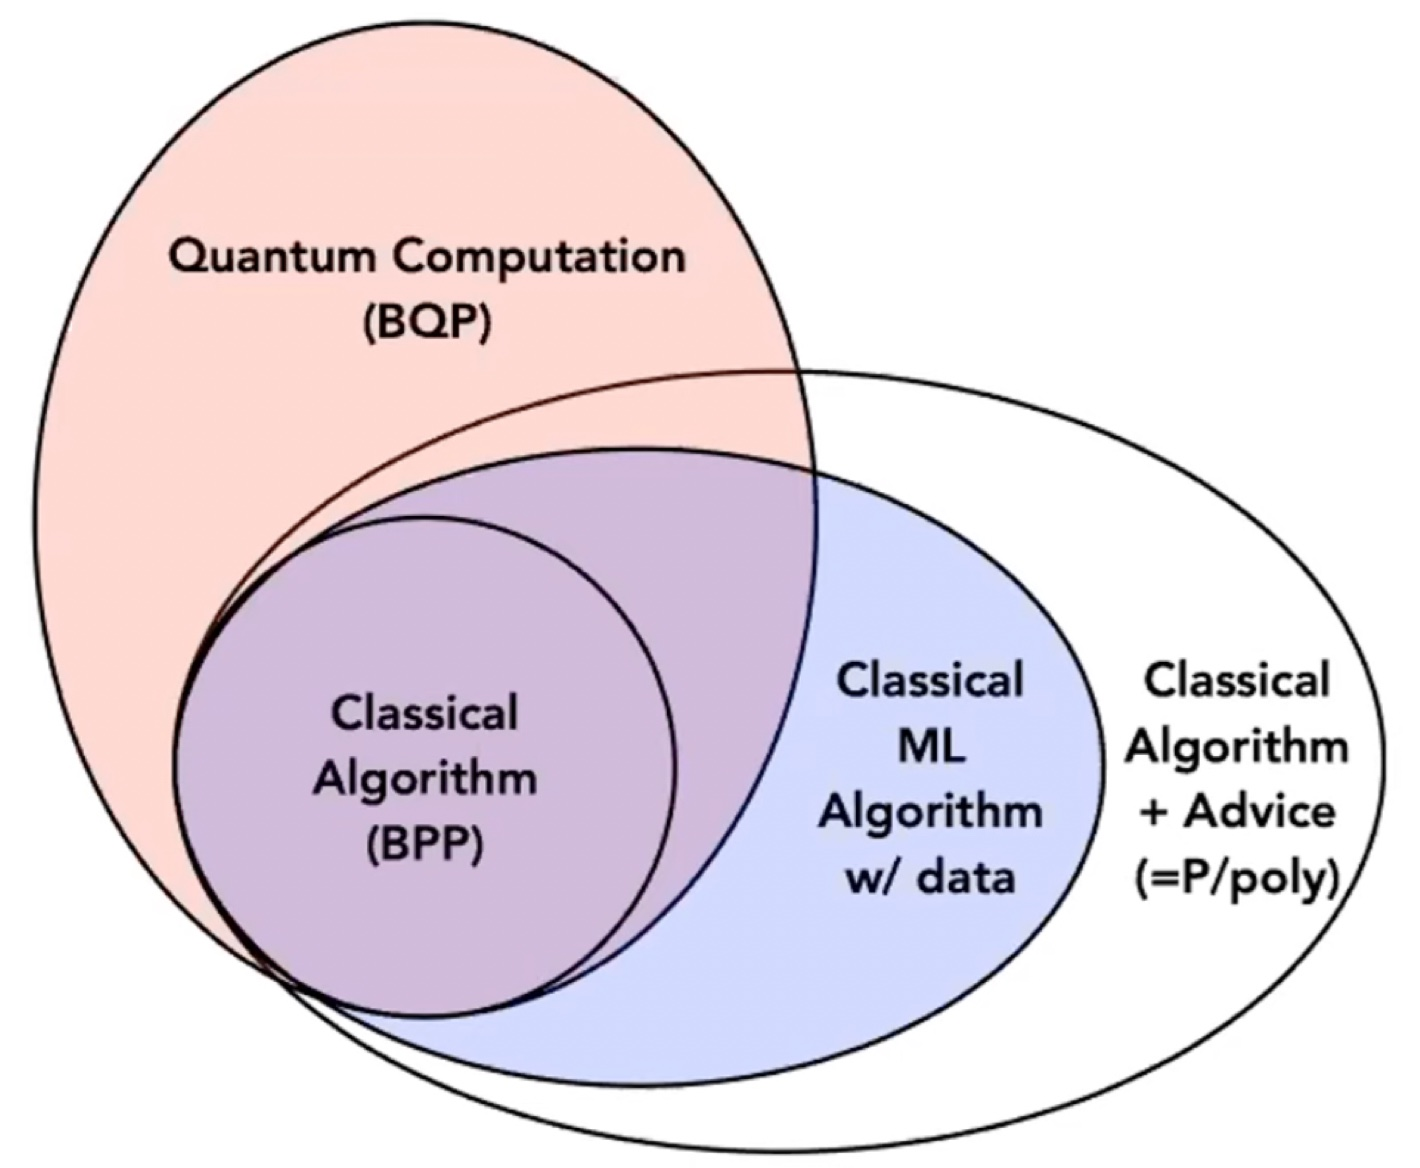
\includegraphics[width=.35\linewidth]{data.jpg}
% 	\caption{computational model powered by training data}
% \end{figure}
power of data - 
\begin{theorem}[informal \cite{huangPowerDataQuantum2021}]
	data learning
	\begin{itemize}
		\item machine learning (strictly) more powerful than BPP
		\item exist quantum advantage in machine learning (not significant, practical)
	\end{itemize}
\end{theorem}
\begin{algorithm}[H]
    \DontPrintSemicolon
    \SetKwInOut{Input}{input}
    \SetKwInOut{Output}{output}
    \Input{labeled features (data), classical shadow?}
    \Output{entanglement structure? decision}
    \BlankLine
    \For{ $i = 1,2, \ldots, m$} {
        kernel estimation \tcp*{a comment}
        % \tcc{comment in a new line}
    {\Return "?"}
    }
    \Return ?
    \caption{Classical learning (SVM)}
    \label{alg:classical_learning}
\end{algorithm}

\subsubsection{Quantum trace (kernel) estimation}
% \begin{definition}[multivariate trace estimation]\label{def:multivariate_trace_estimation}
% 	The task of estimating quantities like 
% 	\begin{equation}
% 		\Tr(\rho_1 \cdots \rho_m)
% 		\tag{multivariate traces}
% 	\end{equation}
% 	given access to copies of the quantum states $\rho_1$  through $\rho_m$.
% \end{definition}
% is a fundamental building block in quantum information science
\begin{theorem}[\cite{quekMultivariateTraceEstimation2022}]
	multivariate \nameref{prm:trace_estimation} can be implemented in constant quantum depth, with only linearly-many controlled two-qubit gates and a linear amount of classical pre-processing	
\end{theorem}

\subsection{Variational quantum circuits}
\subsubsection{Variational quantum kernel estimation}
an ansatz for \nameref{def:entanglement_witness}
\begin{equation}
	\ew_{a} := \sum_{\qty{i\dots}}  a_{..} \bigotimes_i^n \hat{\sigma}^{(i)}
	,\quad \hat{\sigma} \in \qty{\sx,\sy,\sz,\identity_{2\times 2}}
\end{equation}
\begin{algorithm}[H]
    \DontPrintSemicolon
    \SetKwInOut{Input}{input}
    \SetKwInOut{Output}{output}
    \Input{density matrix $\dm$}
    \Output{determine entangled structure??}
    \BlankLine
    \For{ $i = 1,2, \ldots, m$} {
        $W_i$  \tcp*{this is a comment}
        % \tcc{comment in a new line}
    {\Return "separable?"}
    }
    \Return entangled ?
    \caption{Entanglement witness by ...}
    \label{alg:entanglement_witness}
\end{algorithm}

\subsubsection{Variational trace estimate}
find optimal entanglement witness (qunatum circuit?)
\cite{glickCovariantQuantumKernels2021}
% \cite{liuRigorousRobustQuantum2021}
\cite{havlicekSupervisedLearningQuantum2019}
\cite{schuldQuantumMachineLearning2019}

\subsection{Theoretic upper bounds and lower bounds}
\cite{huangPowerDataQuantum2021}
\cite{huangPredictingManyProperties2020}
\cite{aaronsonShadowTomographyQuantum2018}
\cite{huangInformationtheoreticBoundsQuantum2021}
\cite{liuRigorousRobustQuantum2021}
\begin{definition}[graph property]\label{def:graph_property}
	monotone
\end{definition}
\begin{problem}[graph property test]\label{prm:graph_property_test}
\end{problem}
quantum advantages:
\begin{itemize}
	\item no input encoding problem \cite{tangQuantumPrincipalComponent2021} in most quantum machine learning algorithm.
	\item contrived problem (engineered dataset)? for exponential speedup
	% \item convex body query? complexity
\end{itemize}
obstacles: (i)
\begin{table}[!ht]
\centering
\begin{tabular}{c|c|c|c|c}
	& gate/depth/computation & measurements/samples & query? & necessary?sufficient \\  
	\hline
	% \nameref{prm:full_tomography} & & N/A & $\bigO$, Holevo bound $\Omega$ & \\  
	\nameref{prm:shadow_tomography} & & \cref{thm:shadow_tomography} & N/A & \\  
	indirect? direct (no prior), promise & & & & \\  
	% promise (low-rank?), partial, decision? & & & & \\  
	entanglement witness (\cref{sec:entanglement_witness}) & & constant & convex?& \\  
	classical ML + SC (\cref{sec:classical_machine_learning})  & & & & \\  
	quantum (variational) circuits & c-depth? & & & \\  
	\hline
\end{tabular}
\caption{complexity measures of different methods}
\end{table}

\section{Numerical simulation}
\subsection{Classification accuracy}
\subsubsection{Data preparation}
multi-partite entangled state: generate synthetic (engineered) data from

\subsubsection{Results}
performance of different methods: 
% \begin{itemize}
% 	\item shadow tomography: 
% 	\item entanglement witness (no machine learning); 
% 	\item classical machine learning; 
% 	\item quantum machine learning
% \end{itemize}

\subsection{Robustness to noise}
tradeoff between (white noise) tolerance (robustness) and efficiency (number of measurements).
\begin{equation}
	\dm_{\noise}' = (1-p_{\noise}) \op{G} + p_{\noise} \frac{\identity}{2^n}
\end{equation}
$p_{\noise}$ indicates the robustness of the algorithm (witness).
\begin{remark}
	the largest noise tolerance $p_{\text{limit}}$ just related to the \textbf{chromatic number} of the graph.[??]
	\nameref{def:graph_property}
\end{remark}
% \input{complexity.tex}
% \input{optimization.tex}

\section{Conclusion and discussion}
todo: experiment (generation, verification) \cite{luEntanglementStructureEntanglement2018}
% \begin{itemize}
% 	\item experiment (generation, verification) \cite{luEntanglementStructureEntanglement2018}
% 	\item error correction? not benchmark
% \end{itemize}

\subsection*{Acknowledgements}
% \thanks{The author thanks} 
% The author thanks
% TikZiT, QuTip

%\begin{appendices}
    %\chapter{}
%\end{appendices}

% %%%%%%%%%%%%%%%Reference%%%%%%%%%%%%%%%
% % \newpage
% % \printbibliography
\bibliographystyle{apsrev4-2}
%\bibliographystyle{alpha}
\bibliography{ref}

%\begin{widetext}
\onecolumngrid
\appendix

\section{Machine learning background}
% In this work, we restrict ourself to supervised learning (mainly SVM), where we are given a set of labeled data for training to predict labels of new data.
% \subsection{SVM}
\begin{definition}[SVM]\label{def:svm}
	support vector machine (SVM) is designed to
	find a hyperplane (a linear function) such that maximize the margin ...
\end{definition}
\nameref{def:kernel}
% \subsection{neural network}
% \subsection{Unsupervised: PCA}
\section{Hardness assumptions}
\BQP,\BPP

%\end{widetext}

\end{document}